\documentclass{article}
\usepackage{tikz}

\begin{document}

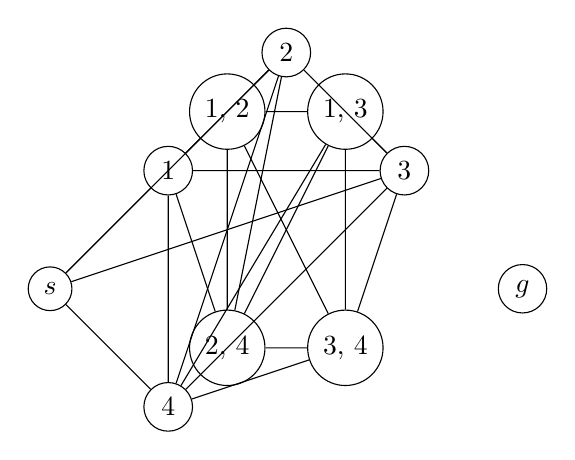
\begin{tikzpicture}[scale=1.5]
    % Define nodes with labels
    \node[circle,draw] (s) at (0,0) {$s$};
    \node[circle,draw] (g) at (4,0) {$g$};
    \node[circle,draw] (1) at (1,1) {1};
    \node[circle,draw] (2) at (2,2) {2};
    \node[circle,draw] (3) at (3,1) {3};
    \node[circle,draw] (4) at (1,-1) {4};
    
    % Draw edges between nodes
    \draw (s) -- (1);
    \draw (s) -- (2);
    \draw (s) -- (3);
    \draw (s) -- (4);
    
    \draw (1) -- (2);
    \draw (1) -- (3);
    \draw (1) -- (4);
    
    \draw (2) -- (3);
    \draw (2) -- (4);
    
    \draw (3) -- (4);
    
    \node[circle,draw] (12) at (1.5,1.5) {1, 2};
    \node[circle,draw] (13) at (2.5,1.5) {1, 3};
    \node[circle,draw] (24) at (1.5,-0.5) {2, 4};
    \node[circle,draw] (34) at (2.5,-0.5) {3, 4};
    
    \draw (1) -- (12);
    \draw (2) -- (12);
    \draw (3) -- (13);
    \draw (4) -- (13);
    
    \draw (1) -- (24);
    \draw (2) -- (24);
    \draw (3) -- (34);
    \draw (4) -- (34);
    
    \draw (12) -- (13);
    \draw (12) -- (24);
    \draw (12) -- (34);
    \draw (13) -- (24);
    \draw (13) -- (34);
    \draw (24) -- (34);
\end{tikzpicture}

\end{document}